\documentclass{article} % 使用 article 文档类
\usepackage{ctex} % 支持中文    
\usepackage[utf8]{inputenc} % 设置输入编码为 UTF-8
\usepackage[T1]{fontenc} % 设置字体编码
\usepackage[english]{babel} % 只保留 english,ctex 会处理中文
\usepackage{amsmath} % 数学公式宏包
\usepackage{amsfonts} % 数学字体宏包
\usepackage{amssymb} % 数学符号宏包
\usepackage{graphicx} % 插入图片的宏包
\usepackage{geometry} % 调整页边距
\geometry{a4paper, margin=1in} % 设置 A4 纸,1 英寸页边距
\usepackage{hyperref} % 添加超链接
\usepackage{booktabs} % 制作表格
\usepackage{float} % 控制图表浮动位置 [H] 强制在此处

% 设置标题、作者、日期
\title{电力需求数据集探索性数据分析报告}
\author{SakuraPuare}
\date{\today} % 使用当前日期

\begin{document}

\maketitle % 生成标题页

\begin{abstract}
本文对 EDS-lab/electricity-demand 数据集进行了初步探索性分析。数据集包含电力需求、元数据和天气信息。分析涵盖了数据量、质量(缺失值、重复值)、关键变量(电力需求 'y', building class, weather variables)的分布,以及变量间的初步关系。报告总结了数据集的主要特征和在进行电力需求预测建模前需要注意的关键问题,如数据分布的右偏、缺失值、天气与需求的时间频率不匹配等。
\end{abstract}

\newpage % 新开一页

\section{引言}
\label{sec:introduction}

电力需求预测是能源领域的重要任务。EDS-lab/electricity-demand 数据集提供了丰富的智能电表数据、元数据和天气数据,为电力需求分析和预测研究提供了基础。本报告旨在通过探索性数据分析 (EDA),初步了解数据集的结构、内容、数据质量以及关键变量的特征和它们之间的关系,为后续的数据清洗、特征工程和模型构建提供指导。

\section{数据集概览}
\label{sec:dataset_overview}

该数据集主要包含三个部分:
\begin{itemize}
    \item \texttt{demand.parquet}: 包含电力需求量 (\texttt{y})、唯一 ID (\texttt{unique\_id}) 和时间戳 (\texttt{timestamp})。
    \item \texttt{metadata.parquet}: 包含每个唯一 ID 的元数据,如地理位置、建筑类型 (\texttt{building\_class})、数据频率 (\texttt{freq}) 等。
    \item \texttt{weather.parquet}: 包含各地理位置随时间变化的天气信息,如温度 (\texttt{temperature\_2m})、湿度 (\texttt{relative\_humidity\_2m}) 等。
\end{itemize}

\section{数据量与数据质量分析}
\label{sec:data_quality}

\subsection{数据量}
\label{subsec:data_volume}
\begin{itemize}
    \item Demand 数据:237,944,171 条记录。
    \item Metadata 数据:7,572 条记录 (对应 7,572 个 \texttt{unique\_id})。
    \item Weather 数据:604,848 条记录。
\end{itemize}

\subsection{缺失值分析}
\label{subsec:missing_values}
\begin{itemize}
    \item Demand 数据:\texttt{y} 列存在约 1.30\% 的缺失值 (3,086,278 条)。其他列无缺失。
    \item Metadata 数据:与地理位置相关的列 (\texttt{location\_id}, \texttt{latitude}, \texttt{longitude}, \texttt{location}) 存在约 3.13\% 的缺失值 (237 行)。其他列无缺失。
    \item Weather 数据:无缺失值。
\end{itemize}
在后续处理中需要决定如何处理 Demand 和 Metadata 中的缺失值。

\subsection{重复值分析}
\label{subsec:duplicate_values}
\begin{itemize}
    \item Demand 数据:未发现基于 \texttt{unique\_id} 和 \texttt{timestamp} 的重复行。
    \item Metadata 数据:未发现基于 \texttt{unique\_id} 的重复行。
    \item Weather 数据:发现了 6 行基于 \texttt{location\_id} 和 \texttt{timestamp} 的重复行 (涉及 12 条记录)。这些重复记录在后续处理中应予以移除。
\end{itemize}

\subsection{时间范围分析}
\label{subsec:time_range}
\begin{itemize}
    \item Demand 数据:从 2011-01-01 00:30:00 到 2017-12-31 23:00:00。
    \item Weather 数据:从 2011-01-01 00:00:00 到 2019-01-01 06:00:00。Weather 数据覆盖了 Demand 数据的时间范围。
\end{itemize}

\section{Demand (电力需求 'y') 分析}
\label{sec:demand_analysis}

通过对 Demand 数据进行 0.5\% 的抽样分析,电力需求量 \texttt{y} 表现出高度的波动性和右偏分布特征。全量数据的描述性统计也证实了这一点 (均值:44.9, 标准差:394.3, 中位数:0.199)。抽样分析发现:
\begin{itemize}
    % 这些是日志中全量 Spark 计算的值,更准确
    \item 均值:约为 44.9 kWh。
    \item 标准差:很大,约 394.3 kWh。
    \item 中位数:仅为 0.199 kWh,远小于均值,表明存在大量小值。
    % \item 极端高值:99\% 分位数约为 681 kWh,而最大值高达 39625 kWh。 (此为抽样值,全量最大值更大)
    \item 极端高值:最大值达到 221,228 kWh。
    \item 非正值:全量数据中约 1.06\% 的非缺失 \texttt{y} 值小于或等于 0。
\end{itemize}
图 \ref{fig:demand_y_dist_orig} 和 \ref{fig:demand_y_dist_log} 展示了抽样数据的分布情况,包括原始尺度和对数变换 (log1p) 后的尺度。对数变换后,分布更接近正态分布,但仍存在一些峰值。这种高度右偏和存在极端值的分布特点需要注意,在建模时可能需要进行数据变换或采用对异常值鲁棒的模型。非正值可能表示零需求或数据采集问题,也需要进一步研究和处理。

\begin{figure}[H] % 使用 [H] 强制图表在此处
    \centering
    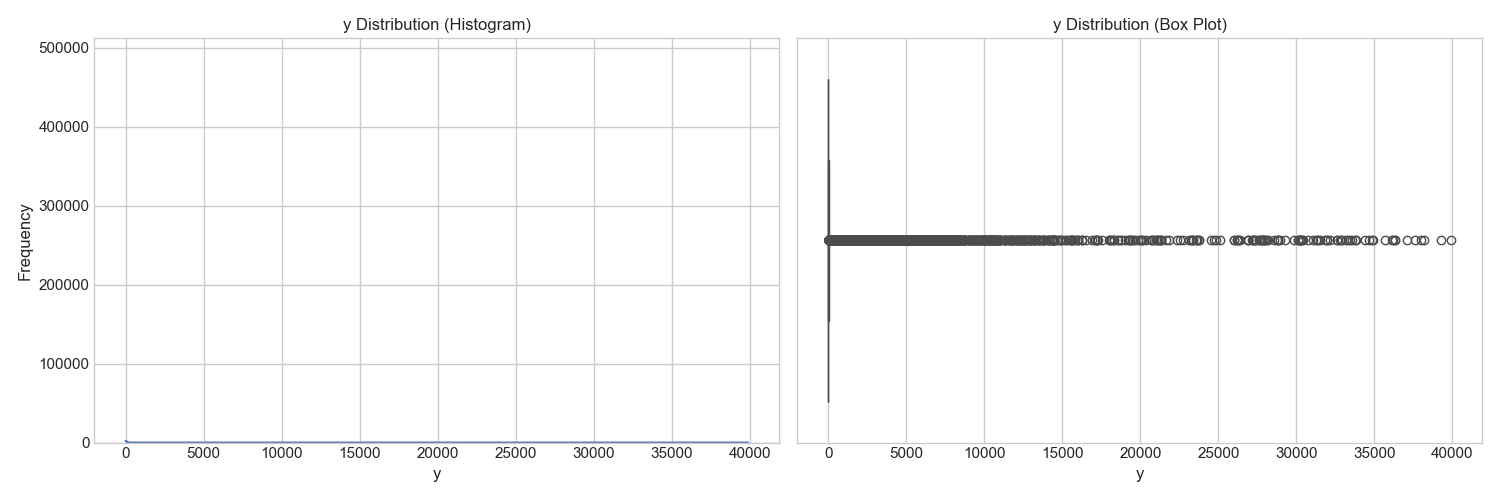
\includegraphics[width=0.8\textwidth]{../plots/Demand Value (y) Distribution (Original Scale, Sample).png}
    \caption{Demand (y) 值分布 (原始尺度,0.5\% 抽样)}
    \label{fig:demand_y_dist_orig}
\end{figure}

\begin{figure}[H]
    \centering
    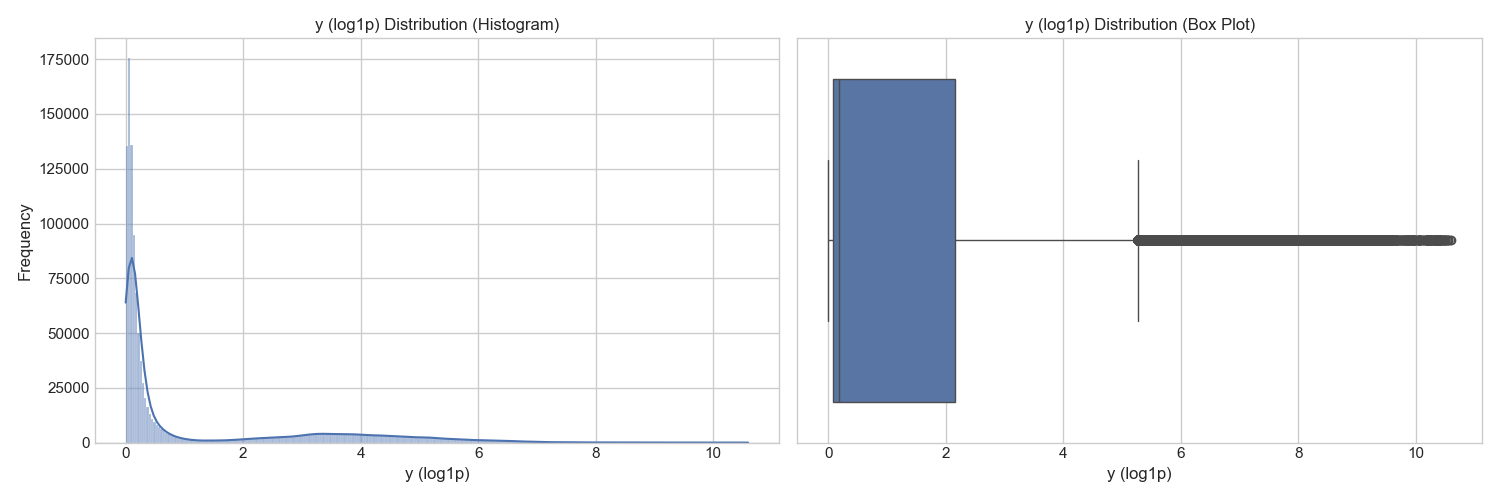
\includegraphics[width=0.8\textwidth]{../plots/Demand Value (y) Distribution (Log1p Scale, Sample).png}
    \caption{Demand (y) 值分布 (Log1p 尺度,0.5\% 抽样)}
    \label{fig:demand_y_dist_log}
\end{figure}

\section{Metadata (元数据) 分析}
\label{sec:metadata_analysis}

元数据提供了每个电表的重要属性信息(图 \ref{fig:metadata_dist_building_class} 到 \ref{fig:metadata_dist_dataset}):
\begin{itemize}
    \item Building Class: 主要为 \texttt{Residential} (5936 个),\texttt{Commercial} (1636 个) 较少。
    \item Location: 主要集中在 \texttt{London, UK} (5634 个),其他地点数量较少,存在 237 个缺失值。
    \item Frequency (\texttt{freq}): 最常见的采样频率是 \texttt{30T} (30 分钟,5566 个),其次是 \texttt{1H} (1 小时,1636 个) 和 \texttt{15T} (15 分钟,370 个)。
    \item Timezone: 主要为 \texttt{Europe/London} (5781 个)。
    \item Dataset Source: 主要来源于 \texttt{London Smart Meter Data} (5566 个)。
\end{itemize}
建筑类型 (\texttt{building\_class}) 是影响电力需求的重要因素。地理位置分布(图 \ref{fig:metadata_location_scatter})显示数据主要集中在英国伦敦区域。

\begin{figure}[H]
    \centering
    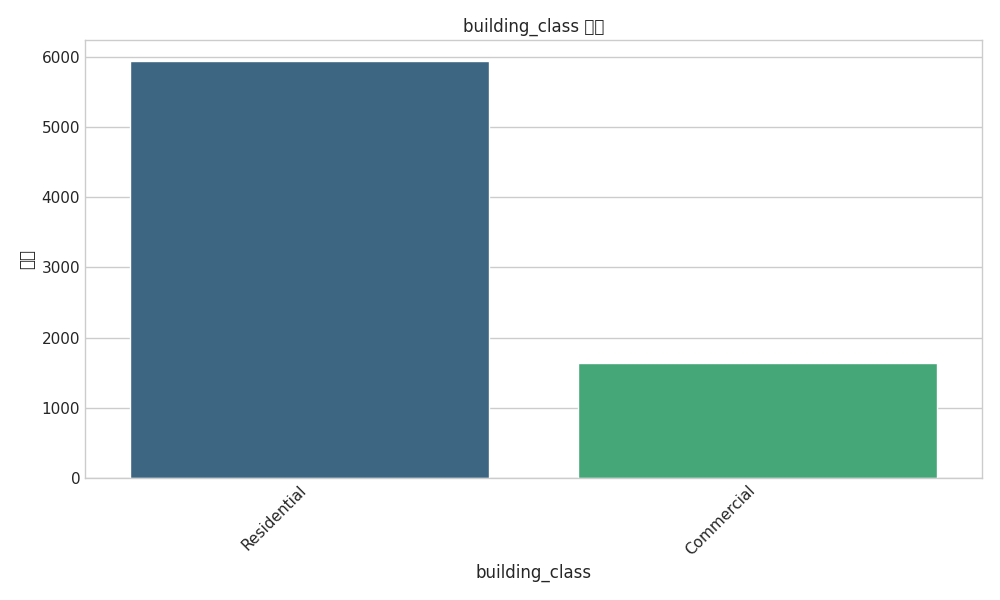
\includegraphics[width=0.6\textwidth]{../plots/metadata_dist_building_class.png}
    \caption{Metadata: Building Class 分布}
    \label{fig:metadata_dist_building_class}
\end{figure}

\begin{figure}[H]
    \centering
    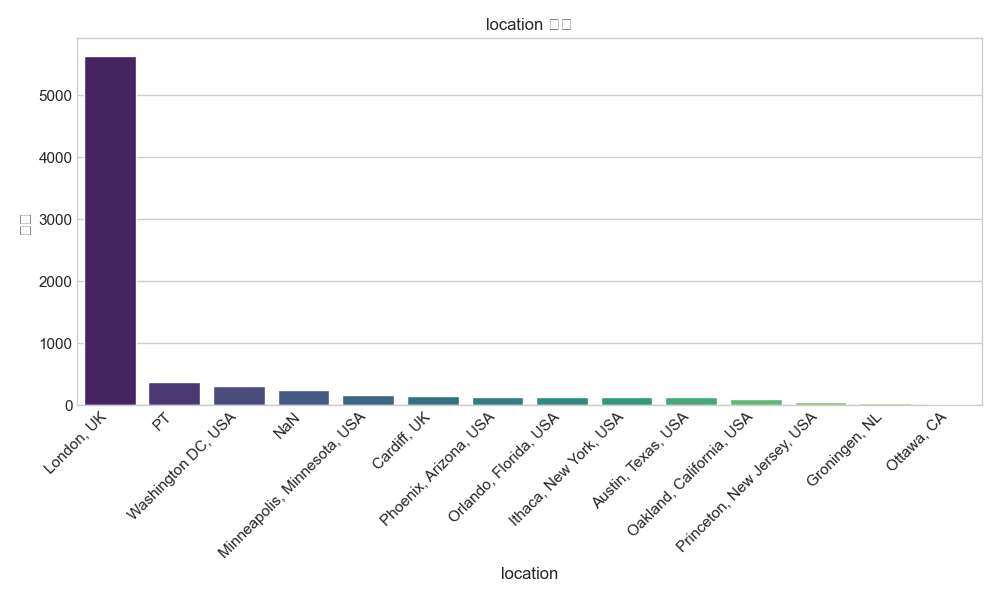
\includegraphics[width=0.8\textwidth]{../plots/metadata_dist_location.png}
    \caption{Metadata: Location 分布 (Top 10)}
    \label{fig:metadata_dist_location}
\end{figure}

\begin{figure}[H]
    \centering
    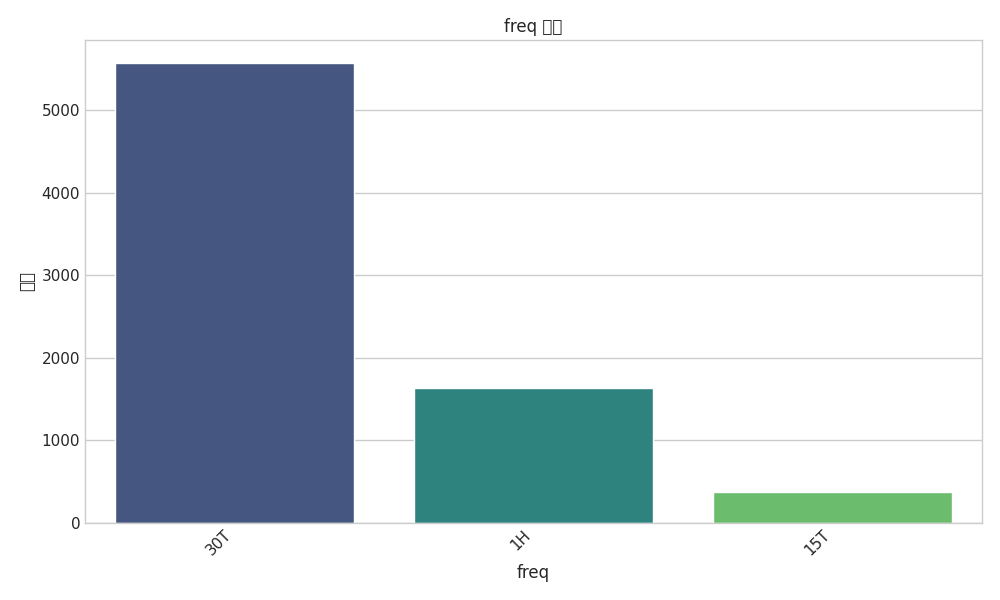
\includegraphics[width=0.6\textwidth]{../plots/metadata_dist_freq.png}
    \caption{Metadata: Frequency (freq) 分布}
    \label{fig:metadata_dist_freq}
\end{figure}

\begin{figure}[H]
    \centering
    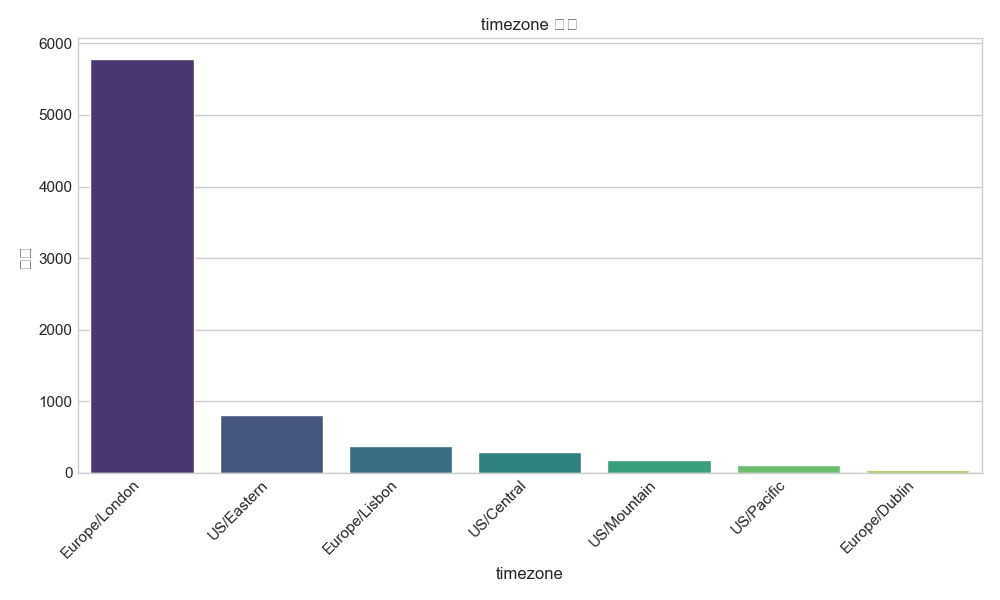
\includegraphics[width=0.7\textwidth]{../plots/metadata_dist_timezone.png}
    \caption{Metadata: Timezone 分布}
    \label{fig:metadata_dist_timezone}
\end{figure}

\begin{figure}[H]
    \centering
    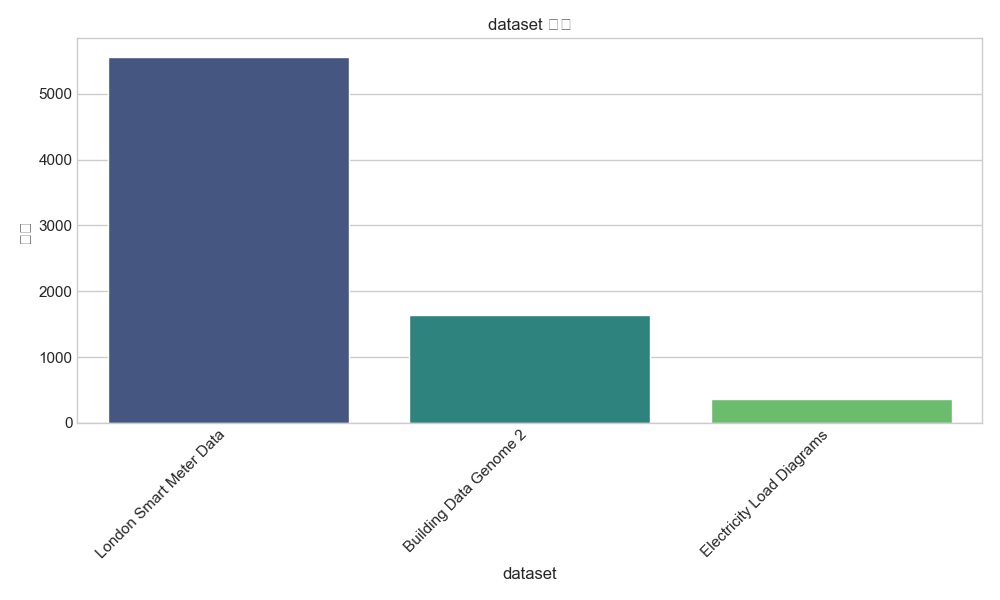
\includegraphics[width=0.7\textwidth]{../plots/metadata_dist_dataset.png}
    \caption{Metadata: Dataset Source 分布}
    \label{fig:metadata_dist_dataset}
\end{figure}

\begin{figure}[H]
    \centering
    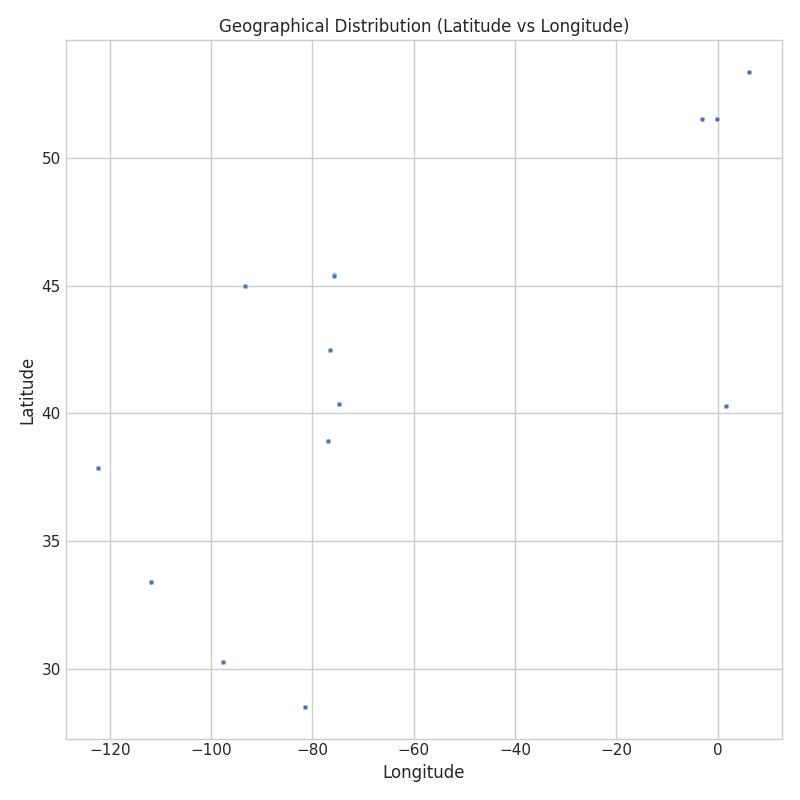
\includegraphics[width=0.7\textwidth]{../plots/metadata_location_scatter.png}
    \caption{Metadata: 地理位置分布 (经纬度散点图)}
    \label{fig:metadata_location_scatter}
\end{figure}

\section{Weather (天气) 分析}
\label{sec:weather_analysis}

天气数据提供了可能影响电力需求的环境因素。关键数值特征(基于完整数据)的描述性统计如下:
\begin{itemize}
    \item \texttt{temperature\_2m} (温度): 均值约 13.0°C,标准差 9.9°C。
    \item \texttt{relative\_humidity\_2m} (相对湿度): 均值约 73.0\%,标准差 19.8\%。
    \item \texttt{precipitation} (降水): 均值为 0.10 mm/h,中位数为 0。
    \item \texttt{wind\_speed\_10m} (风速): 均值约 12.8 km/h,标准差 6.8 km/h。
\end{itemize}
图 \ref{fig:weather_dist_temp} 和 \ref{fig:weather_dist_humidity} 展示了温度和相对湿度的分布(基于 5\% 抽样)。未在 \texttt{precipitation}, \texttt{rain}, \texttt{snowfall} 列中发现负值,数据质量较好。天气代码 (\texttt{weather\_code}) 和是否白天 (\texttt{is\_day}) 的分布见图 \ref{fig:weather_dist_code} 和 \ref{fig:weather_dist_is_day}。

\begin{figure}[H]
    \centering
    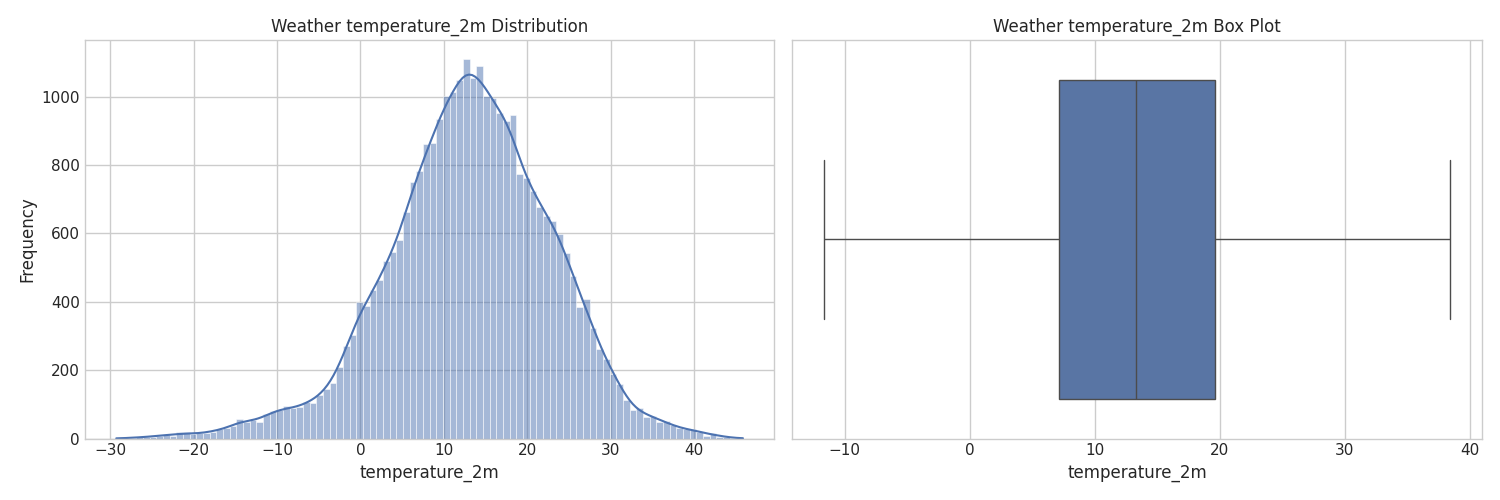
\includegraphics[width=0.8\textwidth]{../plots/weather_distribution_temperature_2m.png}
    \caption{Weather: Temperature (2m) 分布 (5\% 抽样)}
    \label{fig:weather_dist_temp}
\end{figure}

\begin{figure}[H]
    \centering
    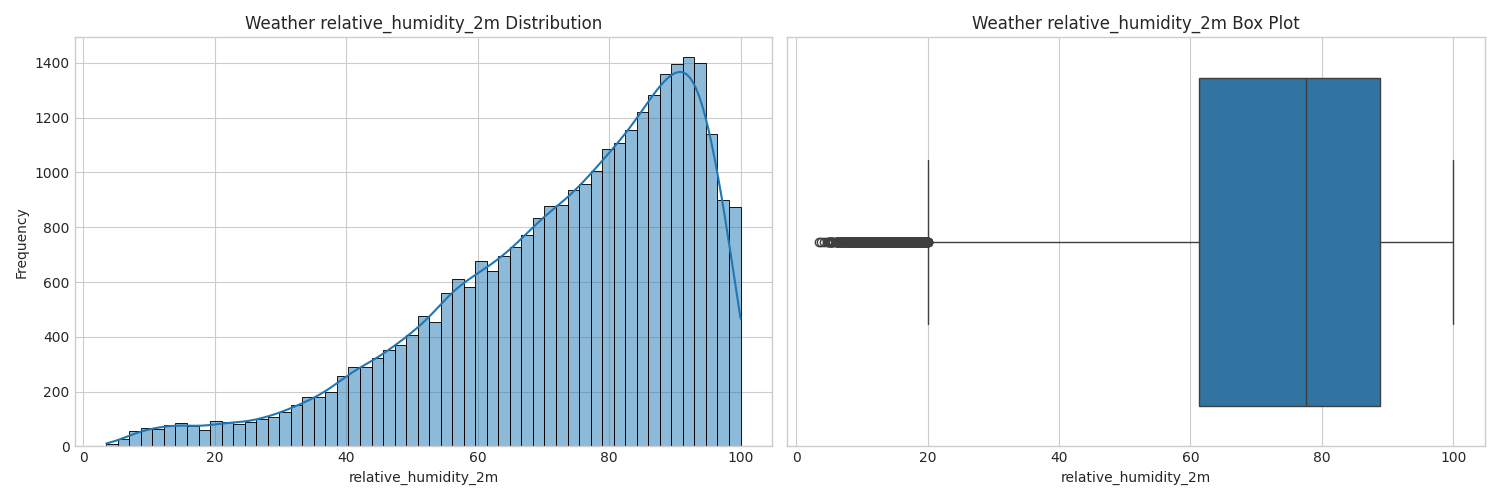
\includegraphics[width=0.8\textwidth]{../plots/weather_distribution_relative_humidity_2m.png}
    \caption{Weather: Relative Humidity (2m) 分布 (5\% 抽样)}
    \label{fig:weather_dist_humidity}
\end{figure}

\begin{figure}[H]
    \centering
    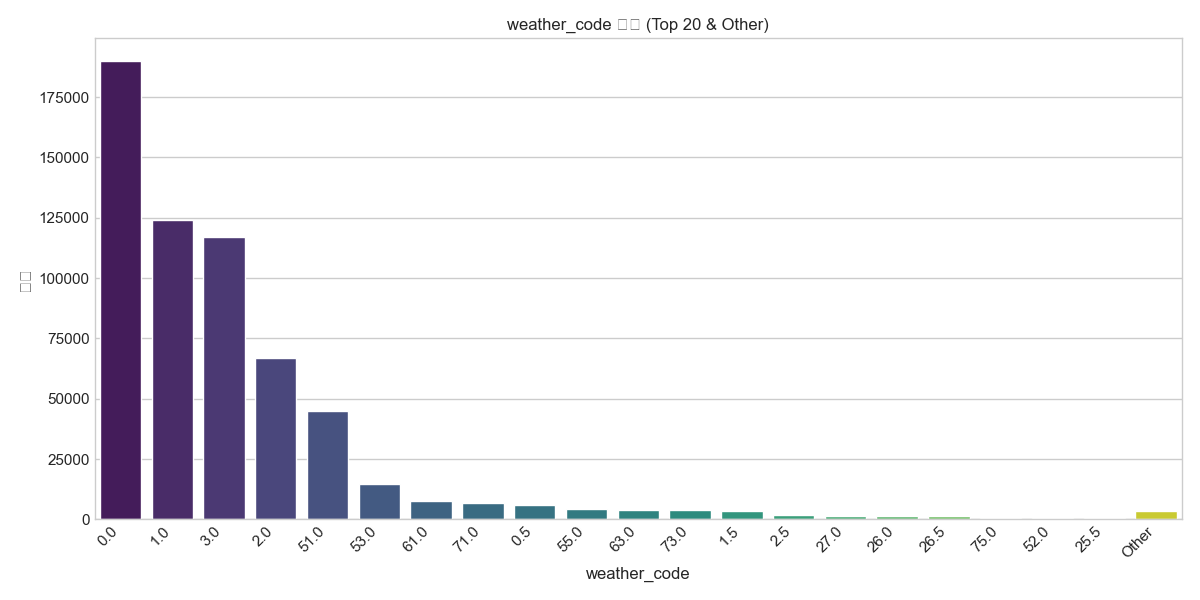
\includegraphics[width=0.8\textwidth]{../plots/weather_dist_weather_code.png}
    \caption{Weather: Weather Code 分布 (Top 20)}
    \label{fig:weather_dist_code}
\end{figure}

\begin{figure}[H]
    \centering
    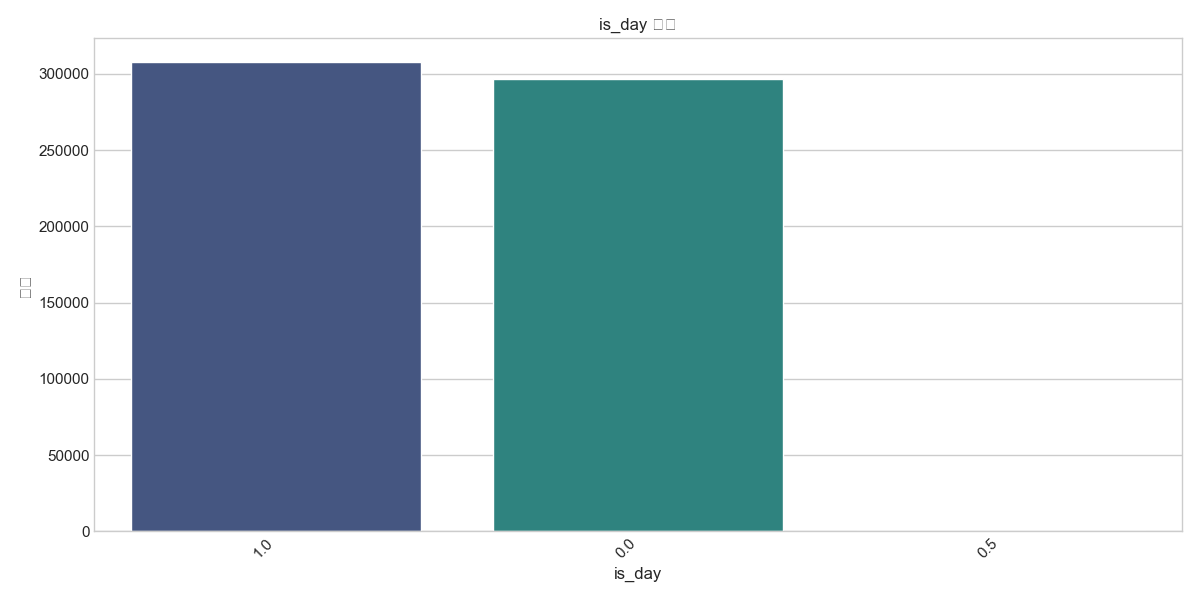
\includegraphics[width=0.6\textwidth]{../plots/weather_dist_is_day.png}
    \caption{Weather: Is Day 分布}
    \label{fig:weather_dist_is_day}
\end{figure}

\section{关系分析}
\label{sec:relationship_analysis}

\subsection{Demand 与 Metadata}
\label{subsec:demand_metadata}
通过对 0.1\% 抽样数据的箱线图分析发现(图 \ref{fig:demand_vs_building_class}),\texttt{Commercial} 建筑的电力需求 (\texttt{y} 值的中位数和分布范围) 通常显著高于 \texttt{Residential} 建筑。对数变换后的图也显示了类似的趋势,但更清晰地展示了低需求区域的分布。这表明建筑类型是预测电力需求的重要特征。类似地,不同数据集来源的电力需求分布也有显著差异(图 \ref{fig:demand_vs_dataset}),这可能与不同数据集采集的建筑类型或地区有关。

\begin{figure}[H]
    \centering
    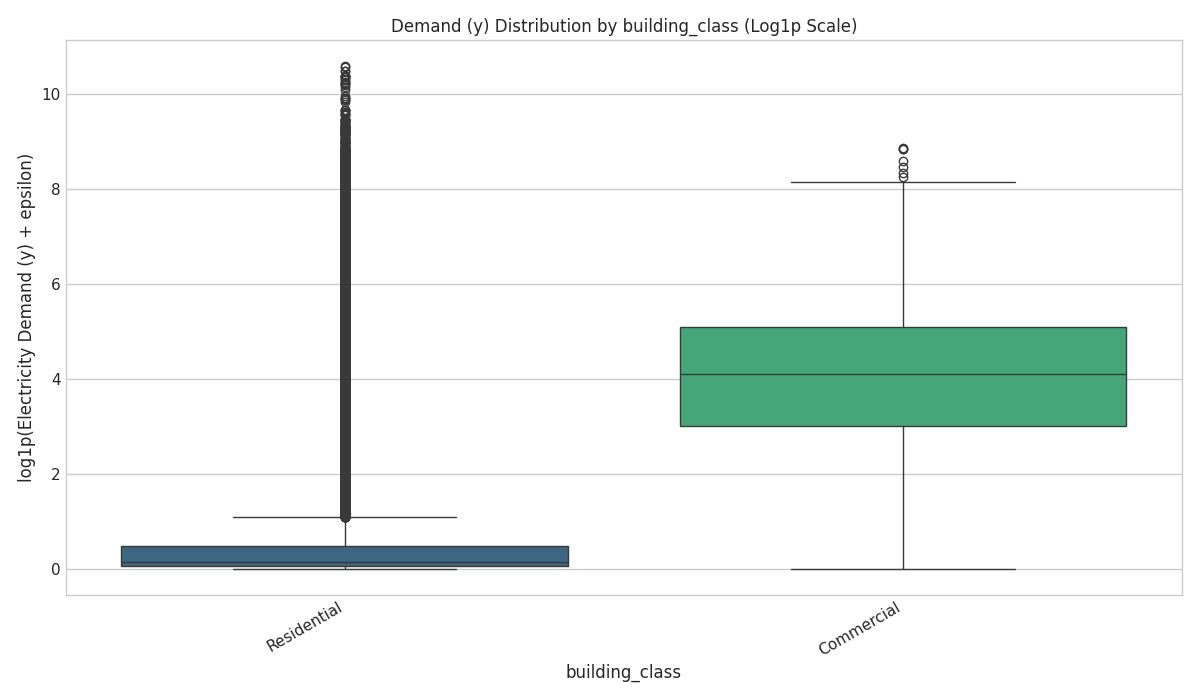
\includegraphics[width=0.8\textwidth]{../plots/demand_vs_building_class_boxplot_log1p.png} % 使用 log1p 图更清晰
    \caption{电力需求 (\texttt{y}, Log1p 尺度) 与建筑类型 (\texttt{building\_class}) 的关系 (0.1\% 抽样)}
    \label{fig:demand_vs_building_class}
\end{figure}

\begin{figure}[H]
    \centering
    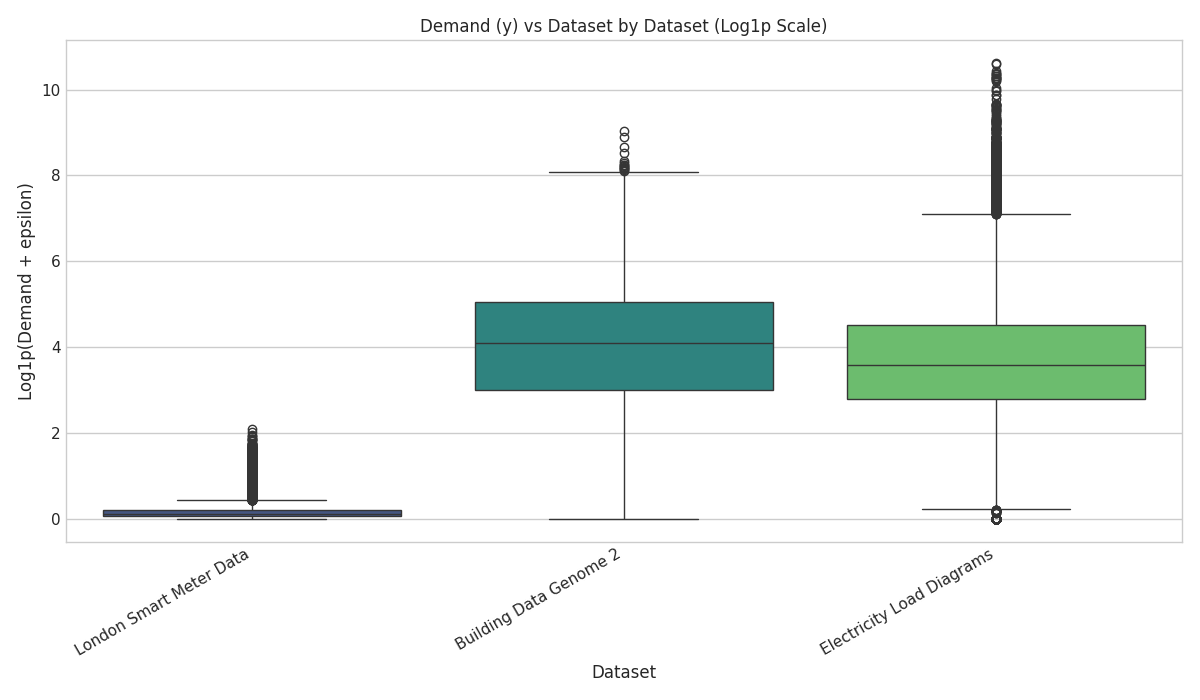
\includegraphics[width=0.8\textwidth]{../plots/demand_vs_dataset_boxplot_log1p.png} % 使用 log1p 图更清晰
    \caption{电力需求 (\texttt{y}, Log1p 尺度) 与数据集来源 (\texttt{dataset}) 的关系 (0.1\% 抽样)}
    \label{fig:demand_vs_dataset}
\end{figure}

\subsection{Demand 与 Weather}
\label{subsec:demand_weather}
基于对 50 个 \texttt{unique\_id} 的抽样数据,并将其与对应的天气数据合并后,计算了电力需求 \texttt{y} 与部分关键天气特征的相关性(基于 Pandas 计算结果):
\begin{itemize}
    \item Demand 与 \texttt{temperature\_2m} 呈正相关 (约 0.334)。
    \item Demand 与 \texttt{relative\_humidity\_2m} 呈负相关 (约 -0.165)。
    \item Demand 与 \texttt{apparent\_temperature} 呈正相关 (约 0.328)。
    \item Demand 与 \texttt{cloud\_cover} 呈负相关 (约 -0.225)。
    \item Demand 与 \texttt{precipitation} (约 0.013) 和 \texttt{wind\_speed\_10m} (约 0.028) 的相关性较弱。
\end{itemize}
这些相关性表明天气因素(尤其是温度、湿度和云量)对电力需求有一定影响。图 \ref{fig:weather_correlation} 展示了天气特征之间的相关性,可见许多天气变量本身高度相关(如温度与体感温度、温度与露点温度等)。

\begin{figure}[H]
    \centering
    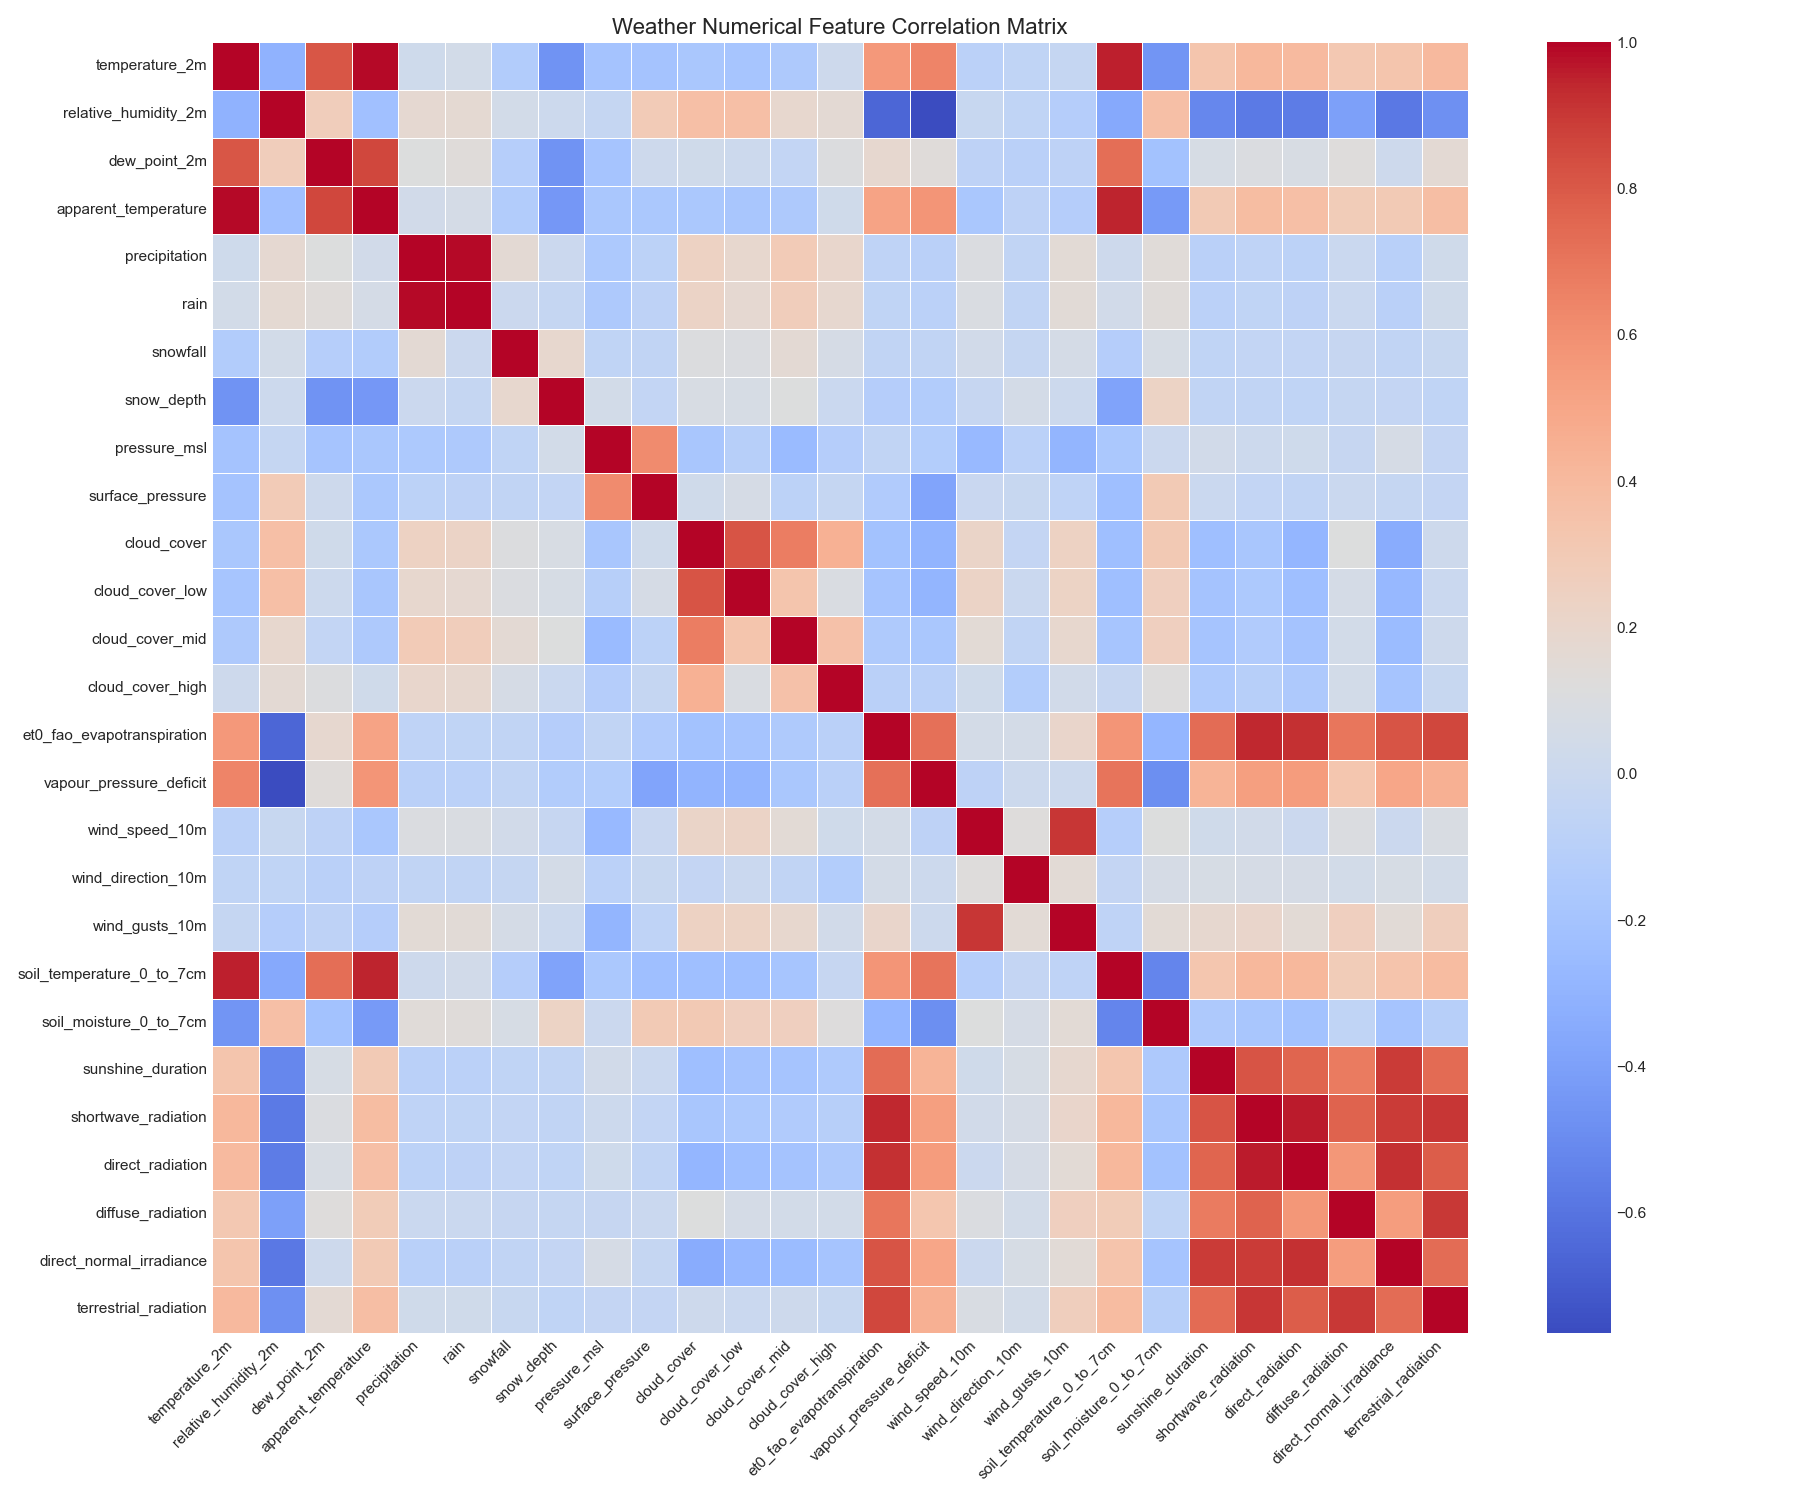
\includegraphics[width=0.9\textwidth]{../plots/weather_correlation_matrix.png}
    \caption{Weather 特征相关性热力图}
    \label{fig:weather_correlation}
\end{figure}

\section{时间特征分析}
\label{sec:time_analysis}

\subsection{时间戳频率分析与匹配}
\label{sec:frequency_matching}
抽样分析显示:
\begin{itemize}
    \item Demand 数据存在多种采样频率,最常见的是 30 分钟 (约 16.8 万样本点),其次是 15 分钟 (约 4.2 万样本点) 和 1 小时 (约 2.8 万样本点) (基于 0.1\% 抽样)。
    \item Weather 数据主要为 1 小时频率 (抽样显示全部为 1 小时)。
\end{itemize}
在合并 Demand 和 Weather 数据进行建模时,需要处理这种时间频率不匹配的问题。常见的方法包括对数据进行重采样(例如,将 15 分钟 和 30 分钟 Demand 数据聚合到 1 小时)或采用适当的插值方法。

\subsection{周期性分析}
\label{sec:periodicity_analysis}
通过聚合分析(图 \ref{fig:demand_by_hour} 至 \ref{fig:demand_by_month}),可以观察到电力需求的周期性模式:
\begin{itemize}
    \item **小时周期**: 平均需求在白天较高,夜间较低,存在早晚高峰。
    \item **星期周期**: 工作日 (周一至周五) 的平均需求通常高于周末。
    \item **月份周期**: 平均需求在冬季和夏季较高,春秋季较低,呈现典型的季节性模式。
\end{itemize}

\begin{figure}[H]
    \centering
    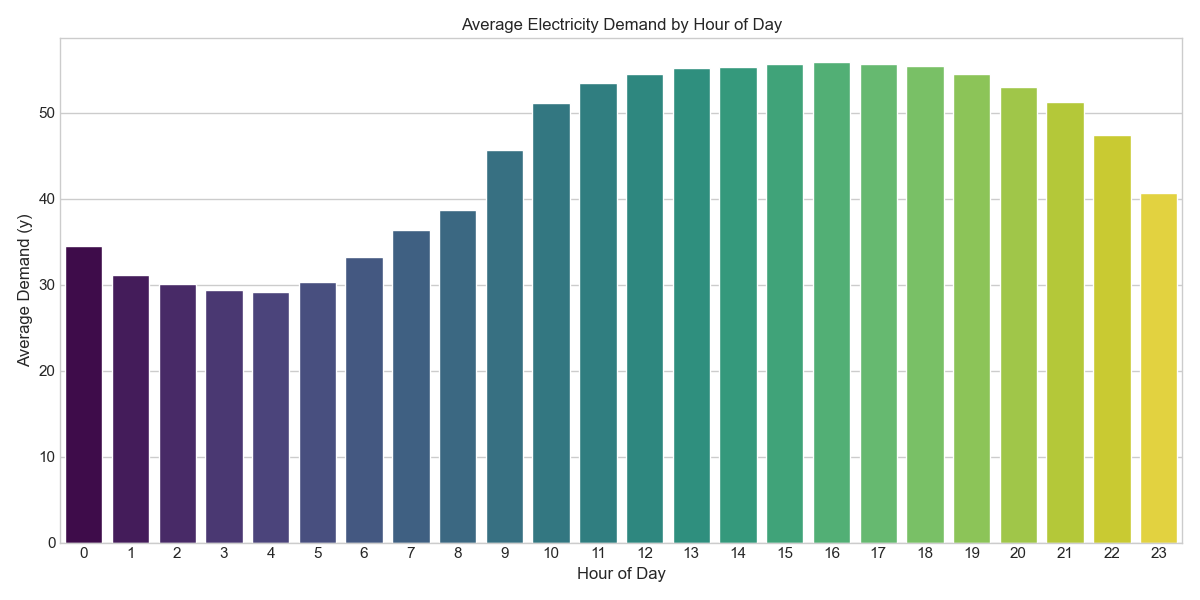
\includegraphics[width=0.8\textwidth]{../plots/avg_demand_by_hour_spark.png}
    \caption{按小时聚合的平均电力需求}
    \label{fig:demand_by_hour}
\end{figure}

\begin{figure}[H]
    \centering
    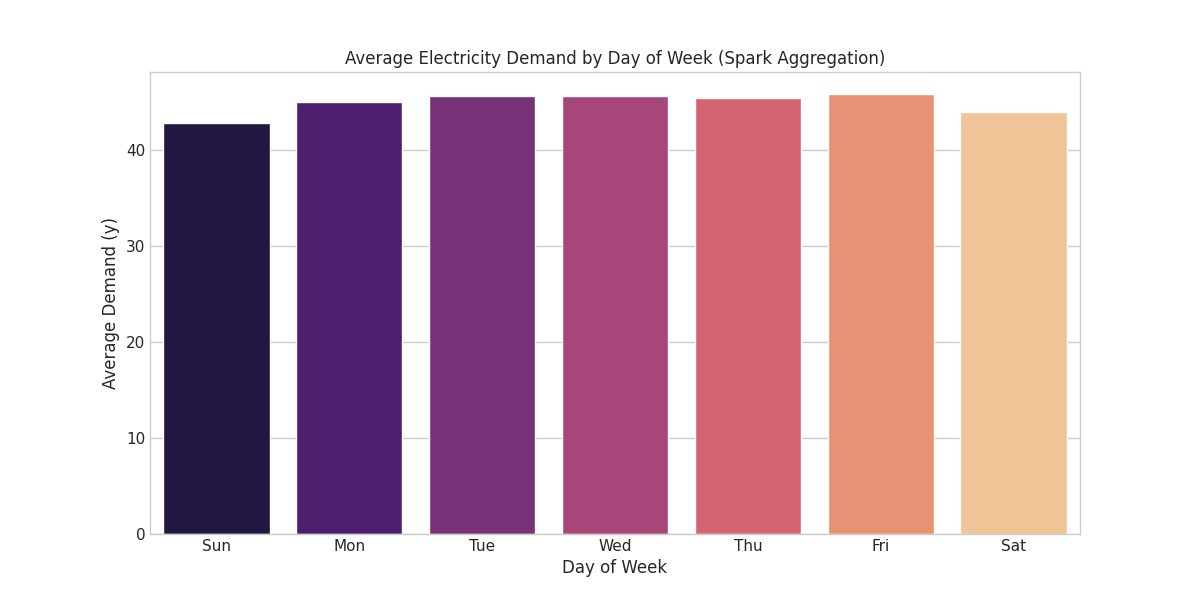
\includegraphics[width=0.8\textwidth]{../plots/avg_demand_by_dayofweek_spark.png}
    \caption{按星期几聚合的平均电力需求}
    \label{fig:demand_by_dayofweek}
\end{figure}

\begin{figure}[H]
    \centering
    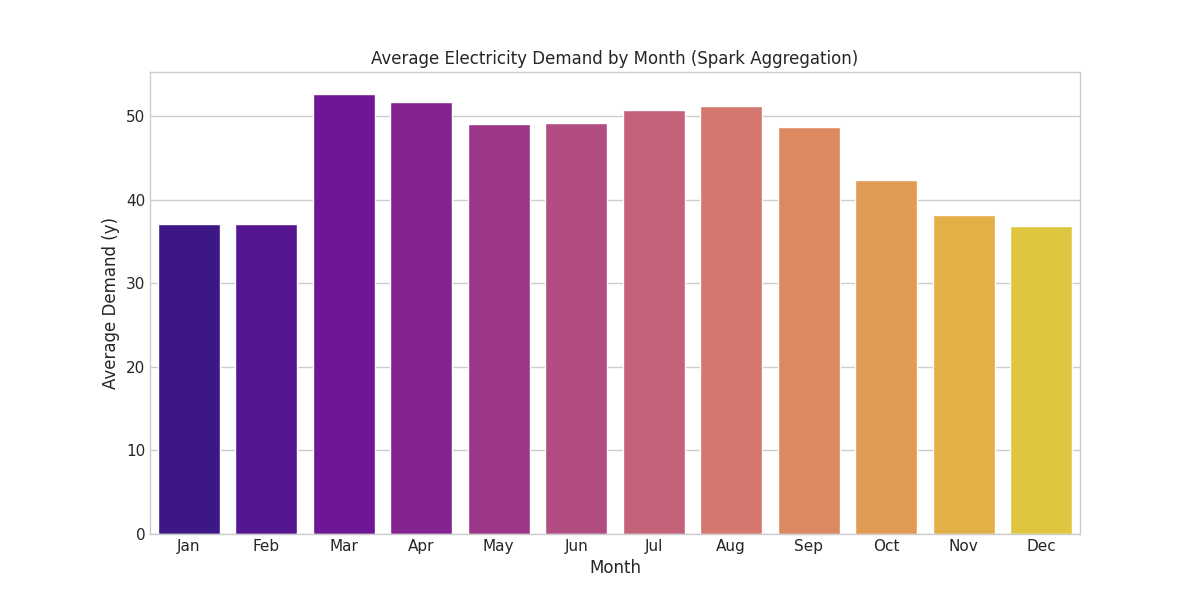
\includegraphics[width=0.8\textwidth]{../plots/avg_demand_by_month_spark.png}
    \caption{按月份聚合的平均电力需求}
    \label{fig:demand_by_month}
\end{figure}

\section{总结与后续步骤}
\label{sec:conclusion}

本次探索性数据分析揭示了电力需求数据集的关键特征和挑战:
\begin{itemize}
    \item 数据量大,包含多源异构数据。
    \item 存在少量缺失值 (Demand: y, Metadata: location) 和重复值 (Weather),需要进行清洗。
    \item 电力需求 (\texttt{y}) 具有高度右偏和极端值,且存在非正值。
    \item 建筑类型、数据集来源、地理位置是影响电力需求的重要类别特征。
    \item 天气因素,特别是温度、湿度和云量,与电力需求存在一定相关性。
    \item 电力需求存在明显的小时、星期、月份周期性。
    \item Demand 和 Weather 数据的时间频率不一致,需要进行对齐。
\end{itemize}

基于以上分析,后续的步骤将包括:
\begin{enumerate}
    \item **数据清洗**: 处理 Demand 和 Metadata 的缺失值,移除 Weather 的重复行,处理 Demand 的非正值。
    \item **时间序列处理**: 将不同频率的 Demand 数据统一(例如重采样到小时),并将 Demand 和 Weather 数据按时间戳和位置进行对齐。
    \item **特征工程**: 基于时间戳提取更详细的时间相关特征 (如小时、星期几、月份、年份、是否节假日、滞后需求等),并合并处理后的天气数据,考虑对高度相关的天气特征进行筛选或组合。
    \item **数据分割**: 根据时间和 \texttt{unique\_id} 构建合适的训练集、验证集和测试集,注意避免数据泄露。
    \item **模型构建与评估**: 选择合适的预测模型 (如 LightGBM, 时间序列模型如 ARIMA/Prophet,或深度学习模型如 LSTM/Transformer) 进行训练、调优和评估,可能需要对 \texttt{y} 进行变换。
\end{enumerate}

本报告为初步分析结果,详细的 EDA 过程和精确数值需要根据完整的分析脚本输出来填充。

\end{document}
